\documentclass[12pt]{article}
\renewcommand{\labelenumi}{(\roman{enumi})}
\usepackage{amsmath, amsthm, amssymb}
% Some extra symbols
\usepackage[bottom]{footmisc}
\usepackage{cite}
\usepackage{url}
\usepackage{graphicx}
\graphicspath{{figures/}} % Graphics will be here
\usepackage{longtable}
\usepackage{hyperref}
\usepackage{setspace}
\usepackage{multirow}
\usepackage{indentfirst}
\usepackage{subfigure}
\usepackage{algorithm}
\usepackage{algorithmic}
\usepackage{listings}
\usepackage{epigraph}
\renewcommand{\epigraphsize}{\footnotesize}
\setlength\epigraphwidth{.48\textwidth}
\usepackage[table,xcdraw]{xcolor}
\setcounter{secnumdepth}{3}
\setcounter{tocdepth}{4}

\usepackage{float}              
\floatstyle{plaintop}           
\restylefloat{table}

\usepackage{booktabs}
\usepackage{dcolumn}
\newcolumntype{d}[1]{D..{#1}}
\newcommand{\mc}[1]{\multicolumn{1}{c@{}}{#1}}



\begin{document}
	% Title Page
	\title{\textbf{CSSM 502} \\ \textit{‘This Music Crept by Me Upon the Waters’}: \\ the Effect of Economic Activity on Listening Habits }
	\author{
		Mahmut Eymen Akın \\
		\\
		\\
		\\
		Submitted to:
		Mehmet Fuat Kına}
	\date{}
	\maketitle{}
	\pagenumbering{roman}
	\pagebreak
	\tableofcontents
	\pagebreak
\section{Introduction}
\begin{epigraphs}
	\qitem{...This music crept by me upon the waters, \newline Allaying both their fury and my passion \newline With its sweet air.}{William Shakespeare, \textit{The Tempest}}
\end{epigraphs}
\pagenumbering{arabic}

Economic circumstances play a major role in determining the well-being of individuals. Times of economic distress are often marked by limited employment prospects, insecure jobs, panics, and significant losses in asset value. Thus, economic downturns affect all citizens of a country, either directly or indirectly. Since it is virtually impossible to isolate entirely from the economic conditions and they limit the actions of individuals at any given time, macroeconomic conditions hold significant sway over the emotional state of the citizens. For instance, people are more optimistic and satisfied during economic booms, and they feel more insecure and stressful during recessions. Bearing this influence of economic activity on emotions in mind, one can observe the reflections of any change in such activity over the emotional outlets where people express themselves. As a major channel of self-expression and emotional catharsis, musical activity is one such outlet. This project aims to unravel the relationship between the economic activity of a country and the emotional content of the music preferred by its citizens. Given the above conjecture, the author expected people to prefer to listen to songs with more positive undertones when the economy is afloat, and listen to songs with bleaker and more somber undertones in times of crisis. However, the initial analyses showed no significant effect.

It is worth noting that the study suffers heavily from several limitations. These include; sample size, lack of covariates, mismatch in the periodic behavior of variables, idiosyncratic factors present in the period of analysis, and last but not least, concerns of endogeneity. Due to time and data constraints, the author has only addressed the sample size and employed a Bayesian approach, which is more robust to smaller datasets. Bayesian analysis resulted in a small negative value, which imply that people tend to listen to more positive songs. 

\section{Literature Review}

This project relies upon a broad literature and aims to bridge them in a coherent application. The related literature can be mainly categorized in two parts: the effects of macroeconomic developments on emotional well-being and the effect of emotions on musical preferences. To the best of the author's knowledge, there is only a single study analyzing the effect of business cycles on musical preferences.

The existent literature on economic downturns demonstrates that recessions cause people to lose their jobs, lead to lower levels of happiness, increase the likelihood of depression and a plethora of other mental health problems, and hamper life satisfaction and optimism on the personal level$^{[1][3]}$. The literature  agrees that economic fluctuations can bring about changes in wages and assets, and thereby lead to stress which affect people's consumption patterns and their overall satisfaction. Main sources of the stress in this context are joblessness, inflation, and negative financial circumstances$^{[4][5][9][11]}$.

The second strand of literature reveals the relationship between the individual's emotional state and its relation to cultural consumption. The relevant body of work suggests a significant correlation between consumption of cultural goods and the emotional circumstances$^{[6]}$. Furthermore, it has been shown that in coping with negative shocks, music is the primary channel through which people console themselves$^{[7]}$. This channel has only gained in significance with the advent of digitization, as it has led the people to increase the variety of their music consumption$^{[2]}$.

The only study that combines these literatures is by Juan de Lucio and Marco Palomeque$^{[8]}$. The paper employs both Natural Language Processing (NLP) algorithms and Spotify audio features analysis to determine the emotional content of popular songs in the United States. The paper checks the response of the average emotional content of weekly top 100 songs to the macroeconomic variables such as unemployment, stock market performance, and inflation rates. The paper suggests that people prefer more positive songs during times of economic stress. This contrast can be most likely attributed to the usage of music as a means of emotional regulation. Studies suggest that people employ music preferences to regulate their emotions during event-related fluctuations, which can be considered as the superset of business cycle shocks$^{[10]}$. This project differs from the study in question in terms of its usage of macroeconomic variables and its coverage, as it extends beyond the United States and analyzes the music preferences of 36 countries. Also, this study differs in terms of employed analysis, as it also includes a Bayesian approach.

\section{Data}

The project utilizes data from various sources. However, prior to that, the project's pipeline will be elaborated. The overarching pipeline is given by Figure 1. 
\begin{figure}[h!]
\centering
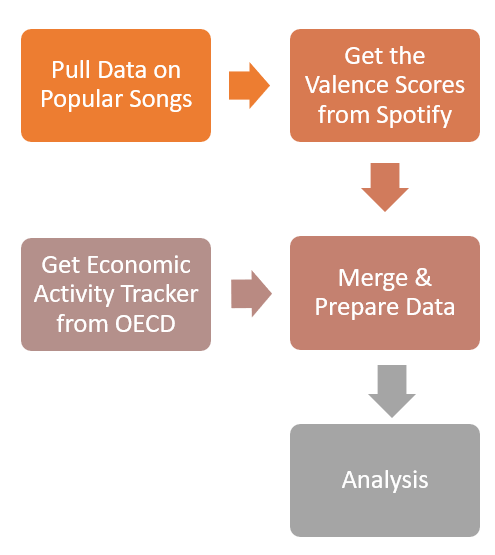
\includegraphics[scale=0.4]{pipeline.png}
\caption{Project Pipeline}
\end{figure}
The initial step consisted of scraping popular songs data from \textit{top-charts.com} on 46 countries over a span of 79 weeks. The website aggregates data from iTunes, Spotify, and YouTube to create their own comprehensive charts. The first recorded week is the 45th week of 2019 and goes on until the 19th week of 2021. For each of these weeks, data on the Top 100 songs were obtained, including song names and their position at the charts. This means 371300 songs in total. These songs constitute the weekly average societal music preferences. Upon obtaining the song data, what remained was to determine the emotional content of these songs to find the emotional circumstances of the countries' citizens. To that end, the project utilizes the track audio features provided by the Spotify's Public API. These include features such as danceability, energy, instrumentalness, etc. The relevant feature for this analysis is the the \textit{valence score}. These scores take a value between 0 and 1 and express the musical positivity of a given track where 0 denotes minimm positivity and 1 denotes maximum positivity. However, to pull valence data from Spotify, a unique song identifier is required, which was not present in the dataset. Thus, the second step in the pipeline composed of separate sub-steps. These include: searching for the name of a track to get its Spotify ID, then using that ID to get its valence score, and then recording it. Since this meant a considerable number of requests to the Spotify's Public API, the author used his discretion to limit the analysis to the Top 10 songs each week. This was due to Spotify blocking both the Developer account credentials and IPs. Even pulling the shrinked 37130 songs required using multiple accounts and IP addresses. Upon getting the songs' valence scores, average weekly valence scores were computed to obtain countries' weekly average emotional conditions. One thing to note here is that since song names came from an alternative source, not all searches returned a song ID, in which case the songs were omitted from the calculation. Similarly, some songs returned an ID but had no features, i.e. Spotify had not analyzed them yet. This was also handled by omitting said songs.

Upon establishing the weekly valence scores per country, the next step required a weekly-observed cross-country indicator of macroeconomic activity. This was possible by relying on the \textit{OECD Weekly Tracker of Economic Activity}, which uses Google Trends data to derive information on consumption, industrial activity, etc$^{[12]}$. The dataset covers 46 countries as well and records both log-deviations in GDP and also the GDP level changes. However, the GDP level measures are all standardized with respect to within-country GDP values for the last quarter of 2019 and therefore are hard to interpret. Thus, the main analyses will rely on log-deviation data. It is worth noting that the 46 countries present in the OECD dataset and the 46 countries present in the \textit{top-charts.com} do not match. The analysis focuses only on countries where both song data and GDP data is present, which comprises of 36 countries. 

\section{Methodology}

The methodology consists of two different approaches. The initial is the frequentist approach where a Panel Data Ordinary Least Squares (OLS) regression is used. However, since sample size may be insufficient to obtain a meaningful variation in the data, an alternative approach is also used. The second is the Bayesian approach. The Panel data regression model can be expressed by the following:
\[
valence_{i,t}=\alpha_i + \gamma_t +\beta_1 \times wGDPdev_{i,t} + \epsilon_{i,t}
\]
where $valence$ denotes the average weekly valence scores, $wGDPdev$ denotes the weekly log-GDP tracker deviations, $\alpha$ and $\gamma$ stand for country- and time-fixed effects, and $i$ and $t$ denote countries and time, respectively.
Although different Bayesian models were employed, the benchmark model can be expressed as:
\[
valence_{i}\sim \mathcal{N}(\beta_0+\beta_1 \times wGDPdev_{i} +\epsilon_{i},\,\sigma^{2})
\]
where $\beta_0 \sim \mathcal{N}(\mu_{\beta_0},\,\sigma^{2}_{\beta_0})$, $\beta_1 \sim \mathcal{N}(\mu_{\beta_1},\,\sigma^{2}_{\beta_1})$, and $\sigma \sim \mathcal{N}(\mu_{sigma},\,\sigma^{2}_{sigma})$. Same parameters denote their analogue versions in this approach. Also, $\mu$'s and $\sigma$'s denote the means and standard deviations of their index parameters, respectively. 

\section{Analysis}

The results of the frequentist analysis can be found in the Table 1 below. In both regressions, we cannot speak of a meaningful effect of weekly economic deviations on the average valence scores of the citizens' musical preferences. 

\begin{table}[!htbp] \centering
	\caption{Panel OLS Results}
	\begin{tabular}{@{\extracolsep{5pt}}lcc} 
		\\[-1.8ex]\hline 
		\hline \\[-1.8ex] 
		& \multicolumn{2}{c}{\textit{Dependent variable:}} \\ 
		\cline{2-3} 
		\\[-1.8ex] & \multicolumn{2}{c}{Valence Score} \\ 
		\\[-1.8ex] & (1) & (2)\\ 
		\hline \\[-1.8ex] 
		Weekly log-GDP deviation & 0.0043 & 0.0216 \\ 
		& (0.0155) & (0.0331) \\ 
		& & \\ 
		\hline \\[-1.8ex] 
		Observations & 2844 & 2844 \\ 
		R$^{2}$ & 2.693e-05 & 0.0002 \\ 
		Country FE & Yes & Yes \\
		Time FE & No & Yes \\
		\hline 
		\hline \\[-1.8ex] 
		\textit{Note:}  & \multicolumn{2}{r}{$^{*}$p$<$0.05; $^{**}$p$<$0.01; $^{***}$p$<$0.001} \\ 
	\end{tabular} 
\end{table} 

This may be due to various reasons. The possible limitations of this study will be explored further in the Conclusions section. However, one possible cause is the small sample size. The Bayesian approach will remedy that, as it is more robust to small sample sizes. The author has tried out multiple models with and without any prior distributions. Also, to check the robustness of the results, different prior distributions were implemented. The results of all models suggested similar results. Figure 2 below gives the convergence of parameter distributions for the models with different priors. 
\begin{figure}[htp]
\centering
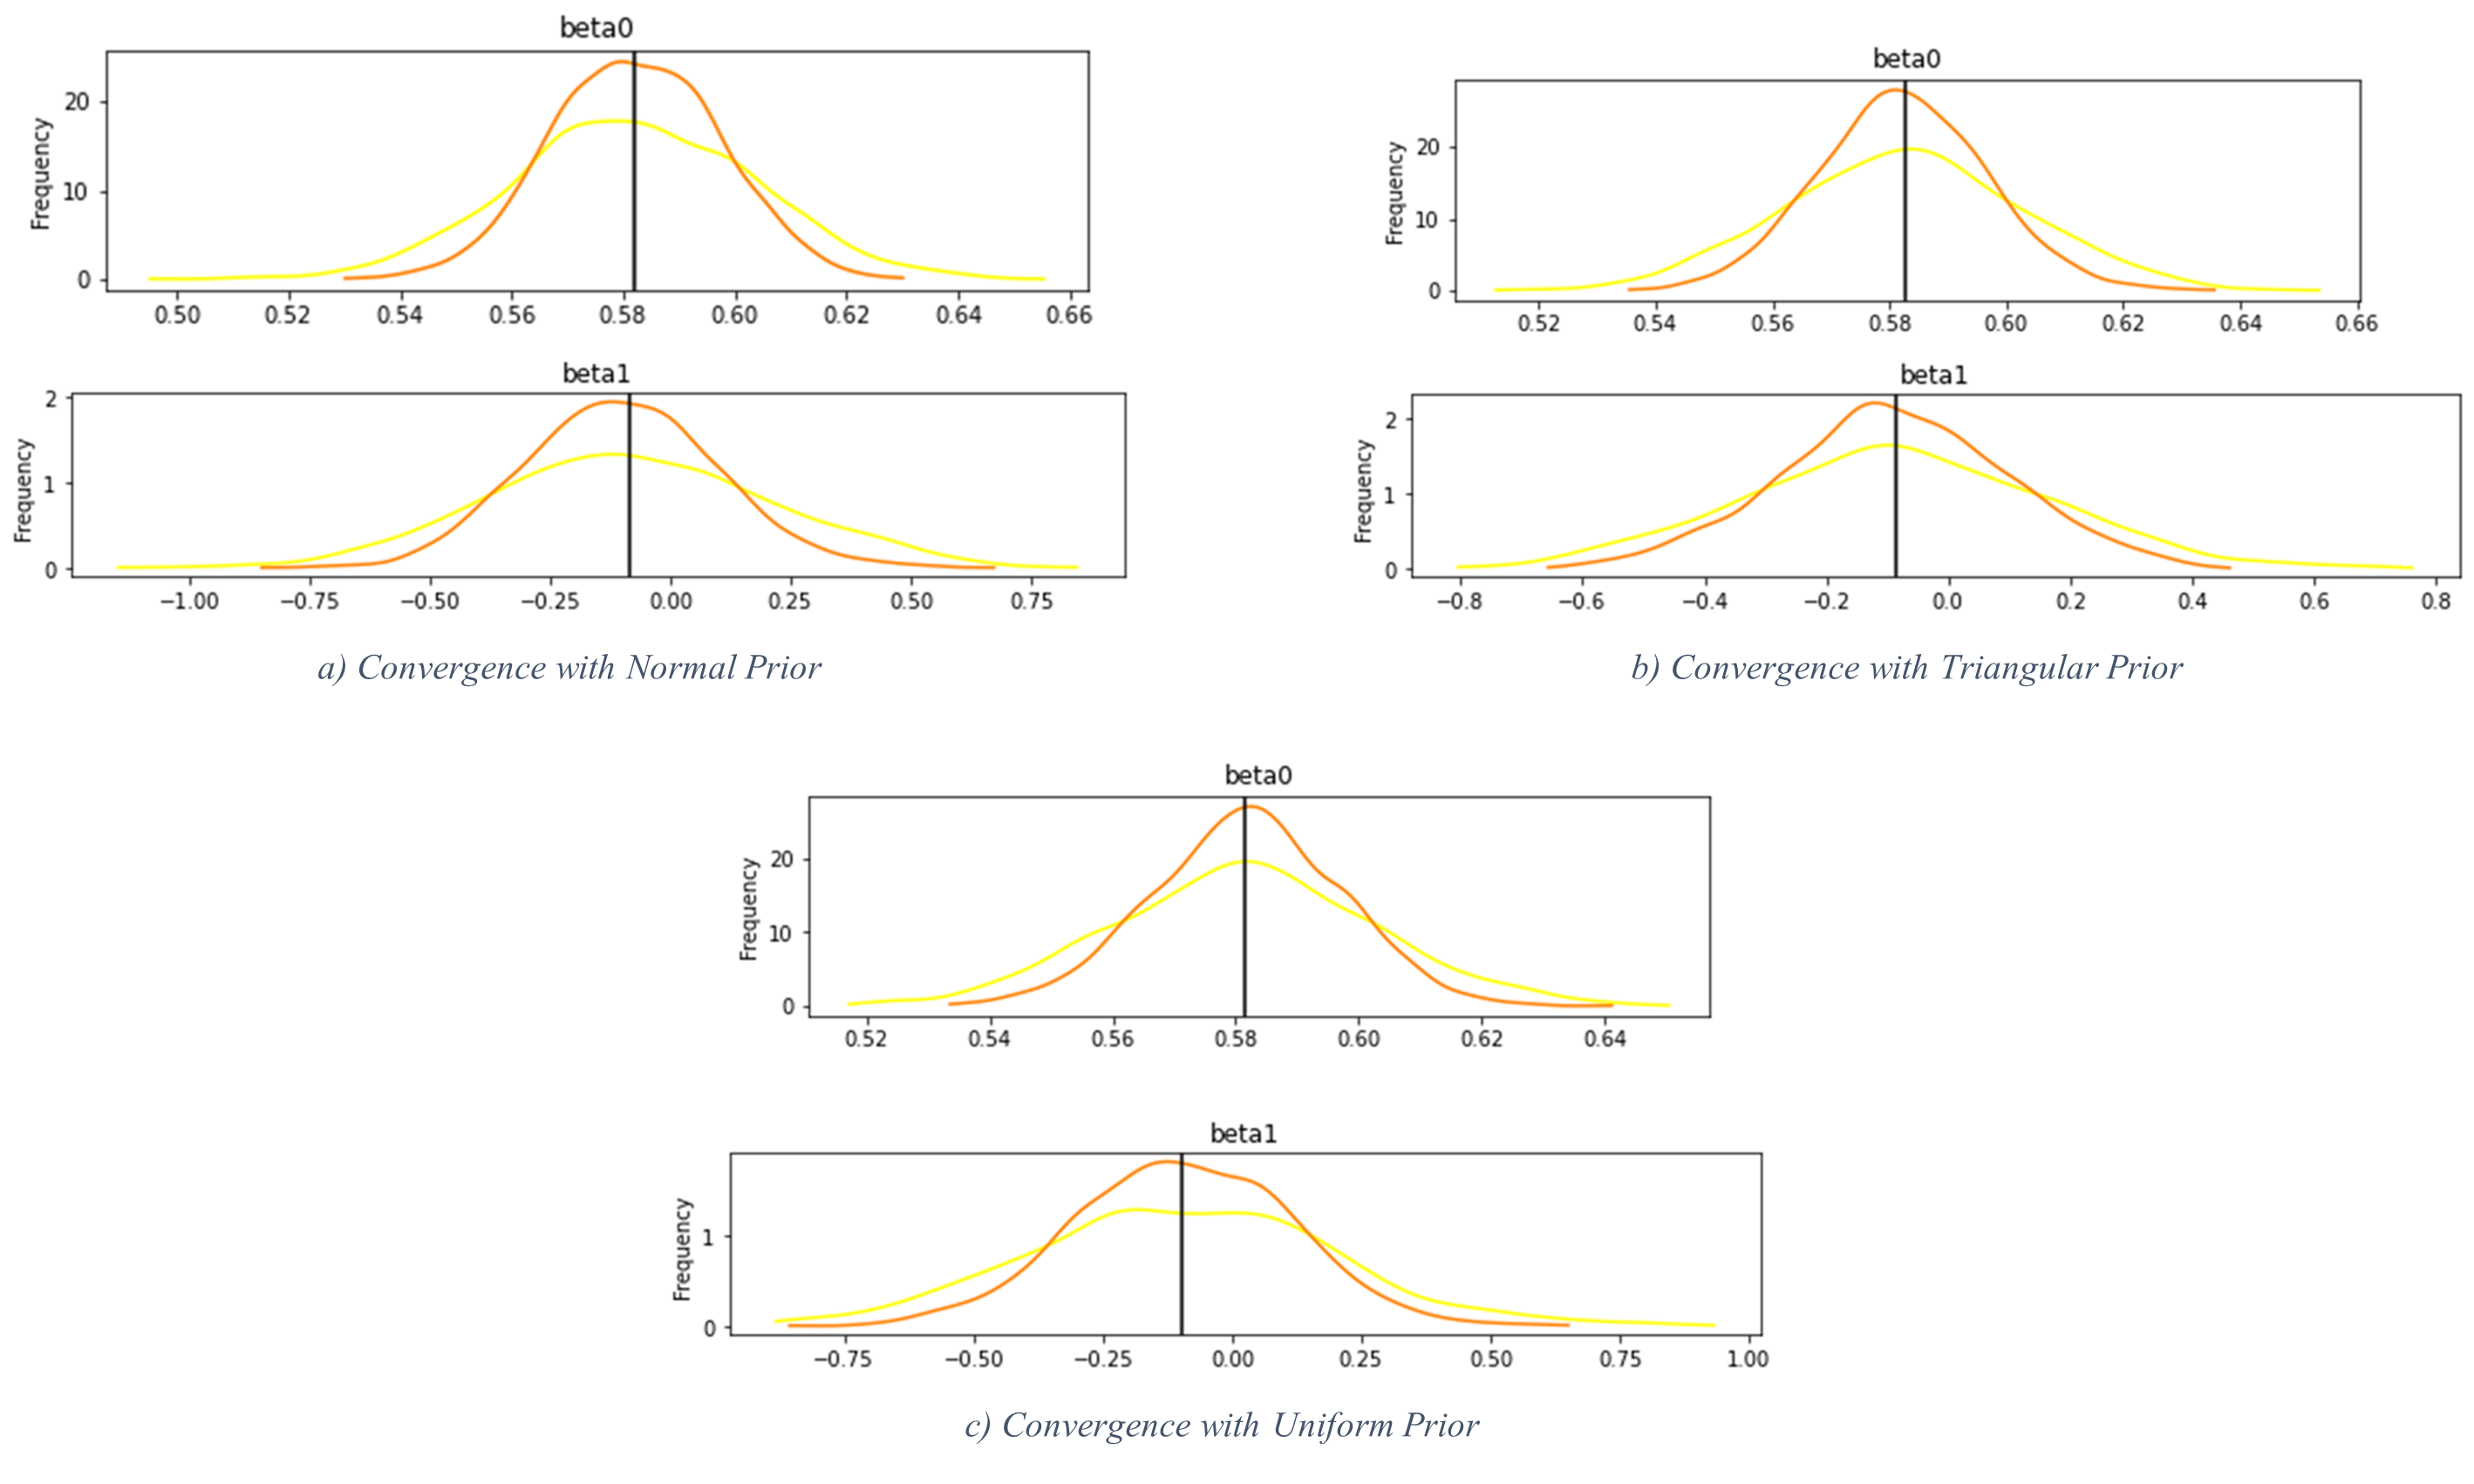
\includegraphics[scale=0.6]{convergence.png}
\caption{Convergence of Parameter Distributions}
\end{figure}

\begin{table}[!htbp] \centering 
	\caption{Bayesian Regression Results}
	\resizebox{\columnwidth}{!}{% 
	\begin{tabular}{@{\extracolsep{5pt}}lcccc} 
		\\[-1.8ex]\hline 
		\hline \\[-1.8ex] 
		& \multicolumn{4}{c}{\textit{Dependent variable:}} \\ 
		\cline{2-5} 
		\\[-1.8ex] & \multicolumn{4}{c}{Valence Score} \\ 
		\\[-1.8ex] & No Prior & Normal Prior & Uniform Prior & Triangular Prior \\ 
		\hline \\[-1.8ex] 
		Weekly log-GDP deviation & -0.092 & -0.084 & -0.097 & -0.084 \\ 
		& (0.023) & (0.296) & (0.296) & (0.254)	 \\ 
		& & \\ 
		Intercept & 0.582 & 0.582 & 0.581 & 0.583 \\
		& (0.002) & (0.022) & (0.021) & (0.020) \\
		\hline \\[-1.8ex] 
		\hline 
		\hline \\[-1.8ex] 
		\\ 
	\end{tabular} 
	}
\end{table} 

As can be observed, the parameter distributions have converged similarly. One thing to note here is that the distributions of the standard errors and the dependent variable are considered as normal in the prior, but the intercept and the coefficient distributions are changed. The results of the regressions are expressed in Table 2 in frequentist terms. It should be noted that the same hypothesis testing applied the Panel OLS will not be valid here. So, the estimated means and standard deviations of parameter distributions should be viewed with caution. However, since in all applications the parameter means have converged to a small negative value, we can conclude that the actual effect will also hold a small negative value around -0.09. Although it is against to the initial expectations of the author, this value is consistent with the results of de Lucio and Palomeque's paper$^{[8]}$. So, one interpretation that can be drawn from this conclusion, people tend to listen to more positive songs during economic downturns, to exert emotional regulation as discussed by Saarikallio$^{[10]}$.

\section{Conclusions and Future Work}

This project aimed to reveal a causal relationship between the economic activity and the emotional content of the societal music preferences. To that end, data from \textit{top-charts.com}, Spotify, and OECD were gathered and analyzed. The analysis adopted two different approaches: the frequentist approach and the Bayesian approach. In the former, a panel data regression with entity- and time-fixed effects was employed and returned insignificant results. On the other hand, the Bayesian approach yielded parameter distributions with a small and negative mean. Also, even in the presence of alternative prior distributions, the results were robust. Thus, in parallel to the existent literature, this project concludes that during economic crises, people tend to listen to songs with more positive sounds. This may stem from people's use of music as a means of emotional regulation under stress. Although the results were contrary to initial expectations, the results add another layer of meaning to the title of this project. Just as the Shakespeare's character \textit{Alonso} is momentarily relieved from his mourning upon hearing a pleasant melody and iterates the passage given in the epigraph, people are pulled towards positive music to allay their concerns.

It should be noted that this study suffers from certain limitations. Firstly, there might be other factors that affect musical preferences and economic activity such as the climate or political conditions. Therefore, there might be serious endogeneity issues in the study. Also, the lack of covariates may imply biased estimates for the frequentist approach. Due to time constraints, other variables could not be integrated into the study. Another important limitation is the period under study. Since the analysis spans late-2019 until mid-2021, it coincides with the Covid-19 pandemic, which probably is a confounding factor. Yet again, since no other sources for country-level weekly songs charts could be found, the project used the sole available data. Another problem is the time periods in analysis. Instead of weekly, economic activity probably exerst more influence on individuals on a monthly or a yearly basis. Nonetheless, using monthly charts would limit the sample size even further. Therefore it was avoided.

\section{References}
\begin{itemize}
	\item[1.] Bell, Brian, et al. “Crime Scars: Recessions and the Making of Career Criminals.” \textit{SSRN Electronic Journal}, 2014, \\*
	https://doi.org/10.2139/ssrn.2468508. 
	
	\item[2.] Bello, P., & Garcia, D. (2021). Cultural Divergence in popular music: the increasing diversity of music consumption on Spotify across countries.
	\textit{Humanities and Social Sciences Communications}, 1(8), 1–8.
	
	\item[3.] Chaves, Covadonga, et al. "The impact of economic recessions on depression and individual and social well-being: the case of Spain (2006–2013)." \\*
	\textit{Social psychiatry and psychiatric epidemiology} 53.9 (2018): 977-986.
	
	\item[4.] Deaton, A. (2012). The financial crisis and the well-being of Americans 2011 OEP Hicks lecture. \textit{Oxford Economic Papers}, 64(1), 1–26.
	
	\item[5.] Frey, B. S., & Stutzer, A. (2010). \textit{Happiness and economics}. Princeton University Press.
	
	\item[6.] Grossi, E., Blessi, G. T., Sacco, P. L., & Buscema, M. (2012). The interaction between culture, health and psychological well-being: Data mining from the italian
	culture and well-being project. \textit{Journal of Happiness Studies}, 13(1), 129–148
	
	\item[7.] Hanser, W. E., ter Bogt, T. F., den Tol, A. J. M. V., Mark, R. E., & Vingerhoets, A. J. J. M. (2016). Consolation through music: A survey study. 
	\textit{Musicae Scientiae}, 20(1), 122–137.
	
	\item[8.] de Lucio, J., Palomeque, M. Music preferences as an instrument of emotional self-regulation along the business cycle. \textit{J Cult Econ} (2022). https://doi.org/10.1007/s10824-022-09454-7
	
	\item[9.] Mertens, A., & Beblo, M. (2016). Self-reported satisfaction and the economic crisis of 2007–2010:	Or how people in the UK and Germany perceive a severe cyclical
	downturn. \textit{Social Indicators	Research}, 125(2), 537–565.
	
	\item[10.] Saarikallio, S. (2011). Music as emotional self-regulation throughout adulthood. \textit{Psychology of Music}, 39(3), 307–327. \\*
	https://doi.org/10.1177/0305735610374894
	
	\item[11.] Wolfers, J. (2003). Is business cycle volatility costly? Evidence from surveys of subjective well-being. \textit{International Finance}, 6(1), 1–26.
	
	\item[12.] Woloszko, N. (2020), “Tracking activity in real time with Google Trends”, OECD Economics Department Working Papers, No. 1634, OECD \\*
	Publishing, Paris, 	https://dx.doi.org/10.1787/6b9c7518-en.
	
	
	
\end{itemize}
\end{document}